\chapter{Introducción}
	
Este primer capítulo describe de forma general la información principal y relevante para poder comprender el funcionamiento del producto actual LUCA, así como los objetivos del proyecto a desarrollar junto con la explicación y motivación del mismo.
	
\section{Introducción}


Dado que el presente trabajo se enmarca dentro del proyecto LUCA, para poder comprender los objetivos de este Trabajo Fin de Grado, se hace necesario describir primero dicho proyecto, lo cual se realiza en la siguiente sección.

\section{LUCA}

\subsection{Motivación}

En los últimos años, el volumen de datos recogidos y manipulados por las empresas ha aumentado de forma vertiginosa. Estos datos se han ido almacenando en diferentes tipos de fuentes conforme las empresas crecían y sus sistemas evolucionaban y se fusionaban. Como resultado de  este proceso no es extraño actualmente encontrar empresas que tengan sus datos almacenados en sistemas tan dispares como bases de datos relacionales, hojas XML o repositorios FTP.


Como consecuencia de esta nueva situación, cuando un usuario quiere obtener una información concreta cuyos datos residen en varios de estos sistemas, éste necesita acceder a cada uno de estos sistemas, extraer de cada sistema la información que precisa, y finalmente filtrarla y unificarla para finalmente obtener los datos requeridos.

Por ejemplo, una cadena de venta de electrodomésticos podría tener sistemas informáticos diferentes para el departamento de atención al cliente, para el departamento técnico de postventa y para el departamento de compras y adquisiciones. Por tanto, para conocer con precisión el estado actual de una reparación, podríamos necesitar:

\begin{enumerate}
	\item Acceder al sistema de atención al cliente para obtener el identificador de la incidencia y en qué fase de su gestión se encuentra.
	\item Una vez corroborado que la incidencia está actualmente siendo atendida, recuperaríamos del sistema de gestión de reparaciones el estado detallado de la reparación. Como resultado de esta operación, supongamos que averiguamos que la reparación está a la espera de recibir una pieza que se ha de sustituir.
	\item Finalmente, para poder hacer una estimación de cuando podría estar lista la reparación, accederíamos al sistema de compra y adquisiciones para averiguar cuando está prevista la entrega de la pieza solicitada.
\end{enumerate}

Como hemos comentado anteriormente, a cada uno de estos sistemas podría accederse de manera diferente. Por ejemplo, el primero podría consultarse utilizando un servicio web. La información del segundo podría recuperarse accediendo directamente a una base de datos relacional, mientras que la información del tercero se obtendría analizando órdenes de compra en formato \emph{pdf} almacenadas en un repositorio de ficheros compartido. Por tanto, el usuario, para poder realizar este proceso, necesita conocer las particularidades de cada sistema y de su forma de acceso.

Para aliviar esta situación, dentro de la empresa CIC, se está desarrollando una aplicación denominada LUCA, a la cual contribuye este Trabajo Fin de Grado. Para facilitar este proceso de recuperación de información, LUCA proporciona un lenguaje común para todas las fuentes de datos a unificar, permitiendo al usuario abstraerse de los detalles de cada fuente.

\subsection{Funcionamiento de LUCA}

A continuación, se detalla brevemente el funcionamiento de LUCA. Para ello, utilizaremos como ejemplo el proceso de recuperación de información de un servicio REST. Concretamente, se utilizará el servicio REST que proporciona información de la flota de autobuses de Santander (TUS). Dicho servicio permite obtener, a partir del identificador de una parada de autobús, información relativa a dicha parada, como, por ejemplo, su localización.

\begin{figure}[!tb]
    \centering
 	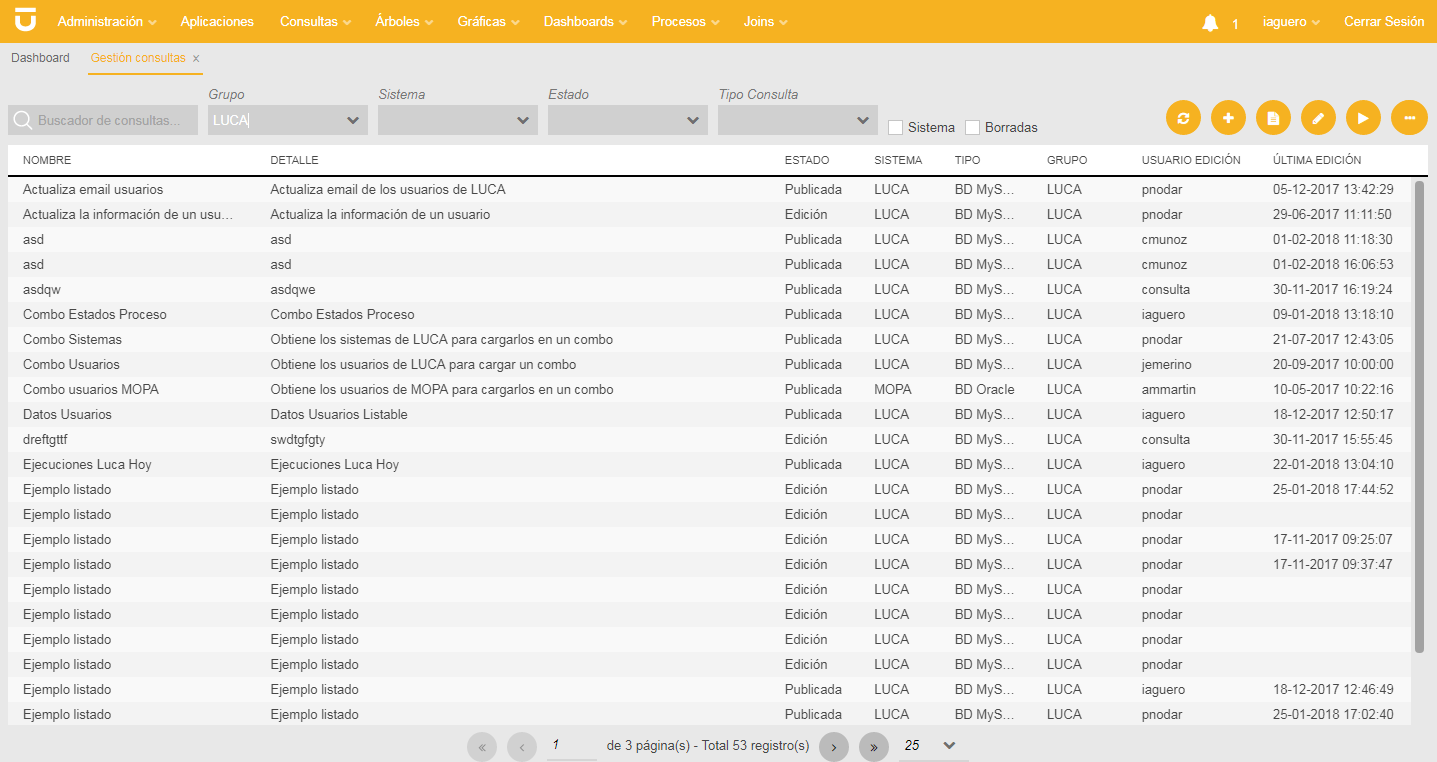
\includegraphics[scale=0.5]{capturasLuca/gestionConsultas.png}
	\caption{Vista de Gestión de Consultas}
    \label{fig:gestionConsulta}
\end{figure}

Al abrir LUCA, nos encontramos con una primera vista (Figura~\ref{fig:gestionConsulta})que proporciona una serie de consultas predefinidas que el usuario tiene disponibles para ejecutar. Estas consultas predefinidas representan procesos de recuperación de información que el usuario realizará habitualmente contra diversos sistemas. En este ejemplo introductorio, se muestran sólo dos consultas: \emph{Flota Estimaciones} e \emph{Información Parada}.


Al seleccionar una consulta, se iniciaría el proceso de ejecución de la misma, para lo cual se abre una nueva interfaz. En primer lugar, debemos proporcionar a la consulta requeriría los datos de entrada necesarios para su ejecución. Por ejemplo, en el caso de la consulta \emph{Información Parada} (Figura~\ref{fig:gestionConsulta}, etiqueta 1) sería necesario proporcionar el identificador de la parada de la que queremos obtener información. Una vez introducido dicho identificador, se seleccionaría el botón de ejecución de la consulta (Figura~\ref{fig:gestionConsulta}, etiqueta 2). La consulta tiene definido internamente cómo acceder al servicio REST, por lo que dicho proceso se realiza de manera transparente al usuario. Finalmente, se muestra el resultado de la consulta, el cuál puede ser visualizado de diferentes formas en función del recurso al que se llama. En nuestro caso, hemos optado por visualizar el resultado de la consulta en formato JSON (Figura~\ref{fig:gestionConsulta}, etiqueta 3).

La principal ventaja que aporta LUCA es que el proceso de ejecución de consultas es opaco para el usuario que la ejecuta. El usuario sólo tiene que proporcionar los parámetros necesarios de entrada y seleccionar un formato de salida. Por tanto, el proceso de ejecución de consultas es exactamente el mismo con independencia de la fuente a la cual se accede.

No obstante, para que dichas consultas pueden ser ejecutadas, cómo llevar a cabo las mismas debe haber sido especificado previamente. Para ello, un usuario con conocimientos suficientes para ello, al que denominaremos en adelante el \emph{creador de consultas}, debe haber especificado cómo ejecutar cada consulta a bajo nivel.

Para poder realizar esta tarea, el creador de consultas accedería a interfaz dedicada a esta tarea (ver Figura~\ref{}). En esta interfaz, definiría primero las variables de entrada y salida de la consulta (Figura~\ref{}, etiqueta 1). A continuación, especificaría cómo llevar a cabo dicha consulta a bajo nivel. Para ello puede utilizar una serie de facilidades y primitivas proporcionadas por LUCA. Para ejemplo, en el caso de la consulta \emph{Información Parada}, utilizando estas facilidades se especificaría el el recurso a obtener y el tipo de llamada HTTP a realizar, un \emph{GET} en nuestro caso.

Lo importante de este proceso es que, una vez definida la consulta, ésta se puede ejecutar fácilmente sin conocer los detalles internos de la misma, incluso hasta el tipo de sistema al que se accede.


	\begin{figure}[H]
		\centering
		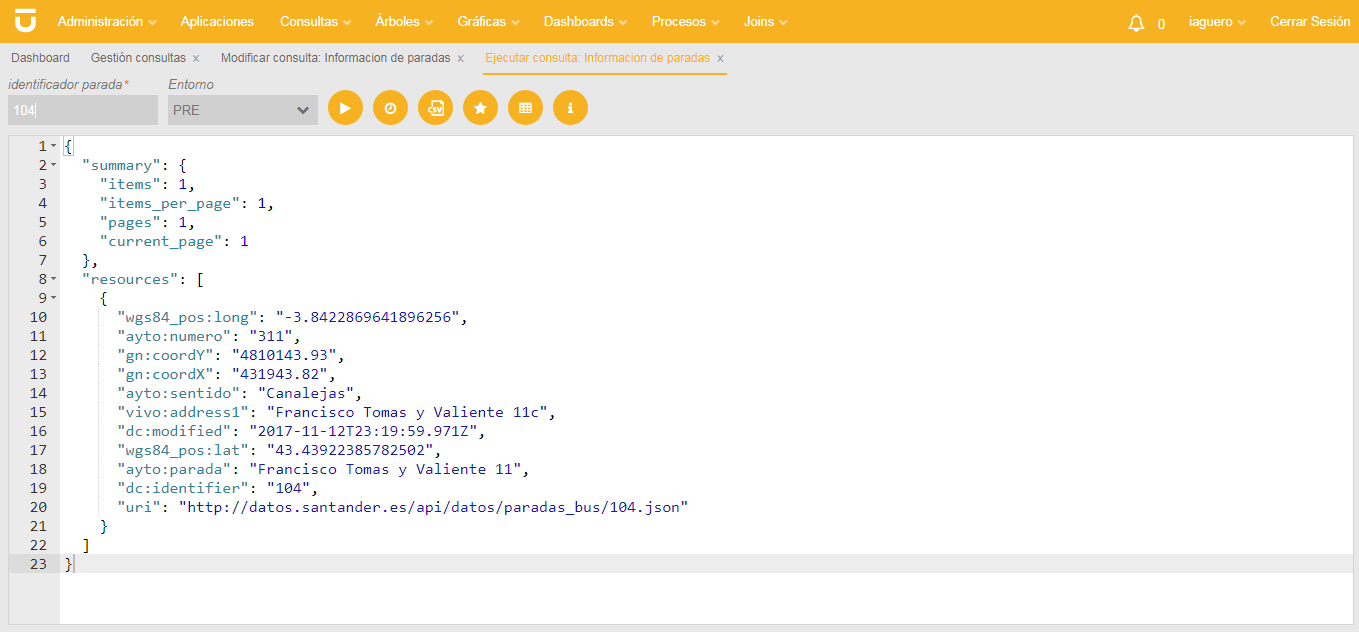
\includegraphics[scale=0.5]{capturasLuca/ejecucionConsulta.png}
		\caption{Vista de Ejecución de Consultas}\label{fig:ejecucionConsultas}
	\end{figure}

\subsection{Limitaciones actuales de LUCA}

Actualmente, LUCA proporciona mecanismos para permitir al usuario recuperar de manera uniforme información de diferentes fuentes de datos. No obstante, LUCA por el momento sólo es capaz recuperar información de una única fuente de datos a la vez. Por tanto, cuando es necesario combinar información procedente de distintas fuentes, el propio usuario es el que debe realizar dicho proceso de composición a mano, ejecutando él cada consulta, y utilizando las salidas de cada una de ellas como entradas para las siguientes.


Un ejemplo de dicho proceso de composición sería la necesidad de un dependiente de una tienda de electrodomésticos de obtener la edad de los usuarios que compraron lavadoras durante el mes pasado. Actualmente, la secuencia de consultas que debería de realizar serían las siguientes:

\begin{itemize}
	\item Primero necesitaría obtener el registro de compras del mes pasado del sistema.
	\item Después, tras guardar dicho registro, tendría que, uno por uno, seleccionar los que se corresponden con lavadoras.
	\item Una vez que el usuario tiene las lavadoras compradas el mes pasado, éste tendría que extraer que usuarios han comprado las lavadoras.
	\item Por último, debería buscar en el sistema cada usuario que ha realizado la compra, a partir del nombre obtenido en el punto anterior, y anotar su edad.
\end{itemize}

En adelante, estas cadenas de consultas para obtener un resultado concreto las denominaremos \emph{procesos}. El problema actual de LUCA, tal como ilustra el ejemplo anterior, es que no soporta el concepto de \emph{proceso}. Por tanto, para ejecutar un proceso,  el usuario tiene que realizar una larga y compleja secuencia de acciones.

\section{Objetivos del Trabajo de Fin de Grado}

El objetivo general de este Trabajo Fin de Grado es integrar en LUCA el concepto de \emph{proceso}. Para ello, hay que dar soporte a dos cuestiones diferentes: (1) la ejecución de los procesos; y (2) la especificación de procesos. Por tanto, el objetivo general de este trabajo se descompone en estos dos subobjetivos principales. 

El primer objetivo implica poder tratar procesos en LUCA de la misma forma que se trata las consultas. Es decir, los procesos deberán aparecer en la interfaz de consultas (ver Figura\ref{}), y ejecutarse mediante el mismo procedimiento utilizado para las consultas simples (ver Apartado\ref{}). Obviamente, la complejidad de ejecutar una proceso es mayor que la de ejecutar una consulta, ya que necesitamos ejecutar varias consultas, guardar resultados intermedios y utilizar estos resultados como entradas para otras consultas.

El segundo objetivo, que es el que implica una mayor complejidad, consiste en facilitar la especificación de procesos en LUCA. Para que un proceso pueda ser ejecutado, primero debe ser especificado, indicando qué consultas lo componen y cómo se relacionan. De acuerdo con los deseos expresados por los responsables del proyecto LUCA y la empresa CIC, dicho mecanismo de especificación debía ser gráfico, permitiendo así componer consultas de manera visual mediante la interconexión de las salidas de unas con las entradas de otras.

Para refinar estos dos grandes objetivos en una serie de requisitos más concretos, se llevó a cabo en primer lugar una reunión con el Jefe y el Gerente del proyecto. El objetivo de dicha reunión era conocer LUCA en profundidad. A continuación, dado que la fase de Ingeniería de Requisitos para este proyecto ya había sido realizada por la propia empresa, se nos proporcionaron unos documentos técnicos con los requisitos técnicos tanto para la ejecución de procesos como para el desarrollo del componente gráfico de especificación de procesos. Estos documentos pueden encontrarse en el Anexo adjunto a la memoria.


Como ya se ha mencionado, en estos documentos se pueden encontrar los requisitos técnicos atribuidos al proyecto, pero, de forma resumida, se centran en tres pilares o requisitos principales:



\begin{itemize}
	\item  Concatenación de las consultas entre si pertenecientes a un mismo proceso.
	\item  Visualización del progreso de ejecución del proceso.
	\item Aplicar criterios de navegación a partir de los resultados de salidas.
\end{itemize}


\section{Arquitectura LUCA}


Esta sección explica la actual arquitectura de LUCA, mostrada en la Figura\ref{} con objeto de que se pueda entender su funcionamiento y cómo el trabajo descrito en este documento se integra en dicha arquitectura. LUCA sigue una arquitectura de tres capas donde la vista de presentación se estructura de acuerdo al patrón \emph{Model-View-Presenter} (MVP).


\begin{figure}[!tb]
	\centering
	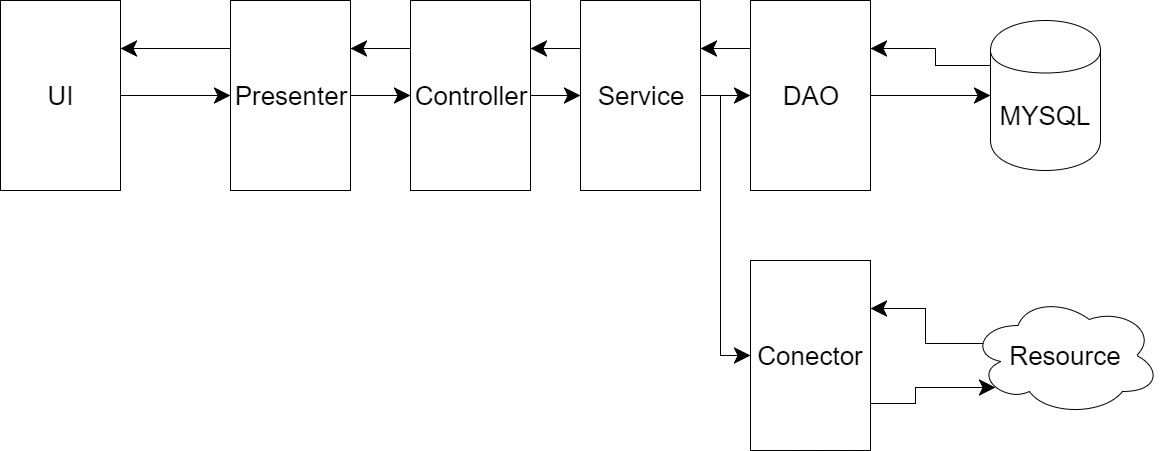
\includegraphics[scale=0.5]{funcionamientoLuca.png}
	\caption{Arquitectura de LUCA}
    \label{fig:funcionamientoLuca}
\end{figure}



\subsection{Arquitectura del Conector}


El conector de LUCA es un componente que se encarga de recibir o recoger los datos de los diferentes recursos albergados en las diferentes fuentes de datos externas. Puede ser de diferentes tipos, como es un conector REST, SOAP o de acceso a bases de datos

En el ejemplo posterior podemos ver un diagrama que describe dicha interacción. El conector en función del tipo va a comunicarse con un cliente diferente, ya sea el HTTPClient \cite{httpclient} de Apache o JDBC \cite{jdbc} de Oracle, para realizar la comunicación y recepción de datos con los diferentes recursos.

\begin{figure}[H]
	\centering
	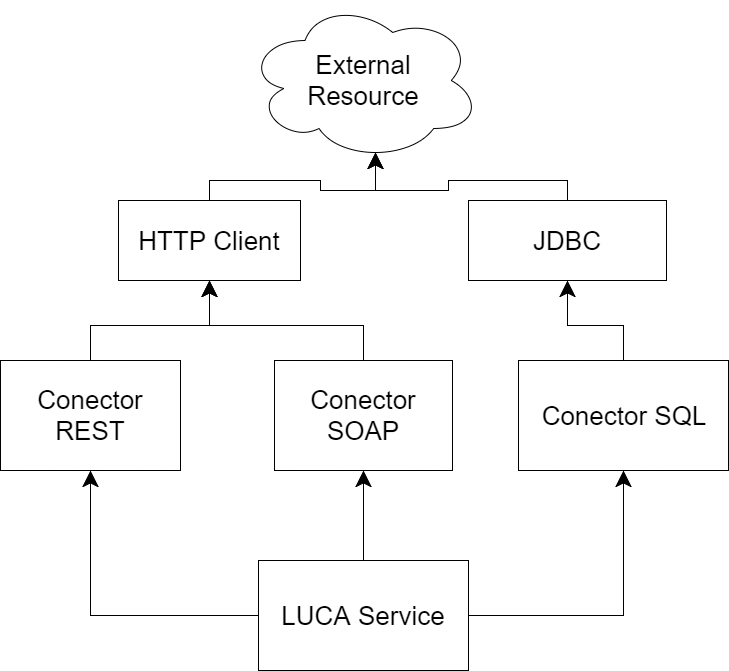
\includegraphics[scale=0.5]{conectorImplementation.png}
	\caption{Arquitectura del Conector}\label{fig:conectorImplementation}
\end{figure}

%%==========================================================================================
%% NOTE(Pablo): ¿Esto de donde sale? Esto es de tu proyecto, no es de LUCA, por lo que
%%   yo no lo mencionaría aquí. Aparte, se entiende regular o nada
%%==========================================================================================

\subsection{Arquitectura del Process-Component}

El Process-Component es un proyecto abstracto (debe de ser importado e implementado por un proyecto o componente padre) encargado de recibir y comunicar los eventos realizados sobre una interfaz construida a partir de la librería GO.JS.

La arquitectura del Process-Component se ostenta en dos pilares. El primero es la implementación de la lógica del propio componente y el segundo es la implementación de un conector que se comunica con una librería de GO.JS que también debe de ser definida.

La lógica del componente se basa en un estado ( el cuál alberga todos los elementos para poder formar la vista), y en una serie de acciones o comandos que se pueden realizar sobre él, y donde tras cada acción, se realiza una comunicación con el conector para que este se encargue de modificar el estado de los elementos de GO.JS.

El conector internamente se compone de la librería encargada de definir el ámbito gráfico con el que se va a trabajar, de una serie de eventos que serán trasladados a la lógica del Process-Component, y de modificar los elementos en activo en la vista bajo la orden especificada.

A continuación, se muestra una figura explicativa de dicha interacción interna entre los componentes:

\begin{figure}[H]
	\centering
	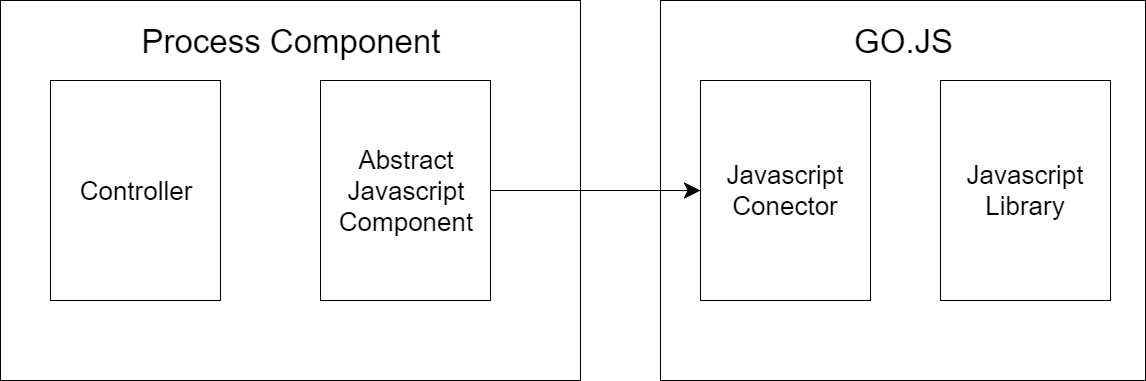
\includegraphics[scale=0.5]{processComponentArquitectura.png}
	\caption{Arquitectura del Process-Component}\label{fig:processComponent}
\end{figure}

Como resumen del funcionamiento del Process-Component, éste es el encargado de recibir eventos realizados sobre la interfaz gráfica, a través del conector hasta llegar a la lógica del componente para publicarlos o abstraerlos a un conjunto de elementos escuchadores que deberán de ser atendidos por el componente implementador de este Process-Component.

%%==========================================================================================
%% NOTE(Pablo): Relacionar esto con los dos subjetivos. Estos dos componentes que se 
%%   mencionan habría que citarlos antes. Esta sección se reescribirá cuando lo anterior
%%   tenga sentido.  
%%==========================================================================================

\section{Planificación}

La sección presente describe el proceso llevado a cabo para realizar el desarrollo tanto del componente gráfico (Process-Component) como del componente de Luca (Luca-Process).

El proceso que se llevó a cabo para realizar el desarrollo del proyecto se basó en dos fases:
	
\begin{itemize}
		\item  Una primera en la que se estudió el funcionamiento de la herramienta gráfica de GO.JS y después se realizó la implementación del Process-Componet.
		\item  Una segunda en la que utilizando el componente descrito anteriormente, se implementa un incremento utilizando la lógica previa de LUCA.
	\end{itemize}

%%==========================================================================================
%% NOTE(Pablo): Esto tan detallado no va aquí y no tiene mucho sentido tenerlo aquí. 
%%   Habría que hablar algo más de que se ha hecho como dos subproyectos diferenciados, 
%%   y que cada proyecto se ha hecho de manera incremental, pero algo informal, sin definir
%%   sprints. Cuando esté claro lo anterior, esta parte te la escribo yo. 
%%==========================================================================================

\subsection{Implementación}
	A continuación se explica brevemente el proceso de implementación llevado a cabo para ambas fases:
	\begin{itemize}
		\item Process-Component
			\subitem El primer paso para empezar la implementación del Process-Component, fue aprender y practicar con ejemplos y con pruebas de concepto para ver como funcionaba y aprender la sintaxis de la librería de GO.JS.
			
			Tras este primer paso, se realizó la implementación del modelo (se puede encontrar en los documentos técnicos), para posteriormente generar una primera prueba de concepto conjunta realizando una comunicación con la librería GO.JS.
			
			
			Por último se implementaron los eventos y escuchadores para posteriormente centrarse en completar dicho componente.
			
			
			
		\item  Luca-Process
			\subitem En este componente se sigue un metodología similar al anterior. Primero se crea una prueba de concepto sencilla para ver la comunicación entre los componentes para posteriormente empezar a montar todo el sistema de recepción de eventos y llamadas al componente gráfico.
			
			\vspace{5mm}
			
			El siguiente paso fue seguir el estilo arquitectónico ya existente en LUCA, utilizando el patrón MVP\cite{mvp} para crear toda la jerarquíca de capas necesarias para la comunicación con los servicios ya existentes de LUCA y la propia base de datos de LUCA.
		
	\end{itemize}


%%==========================================================================================
%% NOTE(Pablo): Esto es demasiado detalle para la parte de planificación. Esto se cometaría
%%   dentro de cada capítulo.
%%==========================================================================================
	
\subsection{Pruebas}

	Este apartado describe el proceso de pruebas llevado a cabo para la comprobación y verificación de las diferentes funcionalidades del proyecto.
	
	\vspace{5mm}
	
	Las pruebas se centraron principalmente en el Luca-Process, ya que es el componente que alberga la mayor lógica del proyecto debido al conjunto de servicios que lo compone y a la lógica sobre los presenters desplegada.
	
	\vspace{5mm}
	
	Profundizando en las pruebas implementadas, solo se han realizado pruebas de integración por varios motivos. El primero es que las pruebas unitarias no son necesarias hacerlas ya que se centran sobre la capa de repositorio y esta capa ha sido implementada con Spring Data Jpa\cite{jpa} y ofrece ya una fiabilidad. El motivo por el que no se realizaron pruebas de sistema, aunque en una primera planificación estaban previstas hacerlas integrandolas con Selenium\cite{selenium} fue la complejidad que lleva la integración junto con Vaadin\cite{vaadin}, ya que la ventaja de programar mediante una captura de eventos sobre la vista toda la secuencia de movimiento sobre dicha vista pasa a ser programática, y debido a que había que ceñirse a unas fechas de entrega y al tiempo que llevaría dicha implementación se decidió omitirlas.
	
	\vspace{5mm}
	
	Las pruebas de integración que se llevaron a cabo se implementaron con Spring Test\cite{springTest} y JUnit\cite{junit}. Desglosando la composición de los mismos, se utilizó en cada test un fichero sql que declaraba las instrucciones de inserción de datos en la base de datos de pruebas necesarios para el correcto funcionamiento de los mismos. La base de datos de pruebas es una base de datos Mysql en local. relacional





	 